
\subsection{Alimentación}
Se eligió utilizar una fuente partida de $\pm60 \ V$  debido a que se buscaba una tensión de salida elevada para obtener un valor de potencia sobre la carga de $\approx 1.5 \ kW$. Para esto, la tensión pico de cada lado del amplificador debe ser de $\approx 53 \ V$. Utilizando $60 \ V$ se llega a un buen compromiso entre tener un margen considerable hasta el recorte para reducir el THD, y el rendimiento del amplificador.\\ 
También se optó por utilizar un segundo riel de alimentación para el par diferencial, teniendo como objetivo optimizar el rendimiento, dado que este trabaja con pequeña señal. Se utilizó un valor de $\pm$ 15V, empleando una resistencia y un diodo zener para proveer esa tensión a partir de la fuente partida principal.
\begin{figure}[H]
\centering
	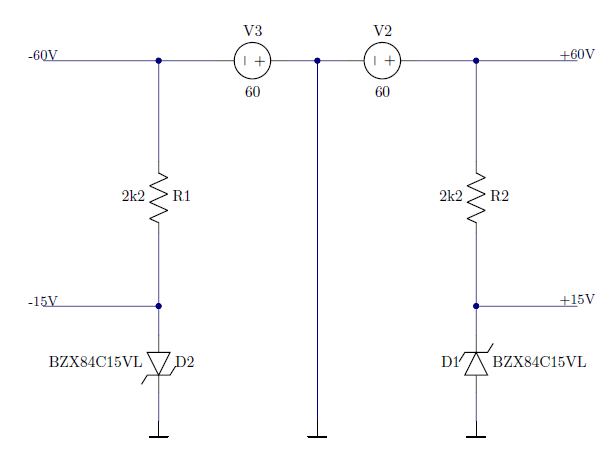
\includegraphics[width=0.7\textwidth]{ImagenesAlimentacion/al.png}
	\caption{Fuente de alimentación}
	\label{fig:alimentacion}
\end{figure}
El diodo seleccionado es uno cuya tensión de zener es de $15 \ V$.
Para el cálculo de la resistencia del diodo se tuvo en cuenta que el diodo quede polarizado con una corriente de mantenimiento de $6 \ mA$ al igual que haya suficiente corriente para que el par diferencial utilice. Teniendo en cuenta la corriente de polarización del par diferencial se llega a la conclusión de que la corriente por la resistencia debe ser de $20 \ mA$.
\begin{align}
R1=\frac{60-V_z}{20mA}= 2k2\Omega
\end{align}
